\subsubsection{Работа с токеном JWT}
Для передачи и обновления токена JWT в сессии используется функция обратного вызова \textit{jwt}, принимающий параметр \textit{trigger}, позволяющий определить сценарий обработки. Логика работы примерно следующая: при первом входе пользователя (\textit{trigger = signIn}) в токен записываются поля \textit{access\_token}, \textit{refresh\_token} и прочие метаданные; при последующих запросах проверяется срок жизни \textit{access\_token}, и при необходимости инициируется процесс его обновления (\textit{trigger = update}). Если же токен ещё валиден, возвращается неизменённая структура. Пример реализации приведён в листинге~\ref{lst:jwt-callback}.

\begin{lstlisting}[caption={Функция обратоного вызова jwt}, label={lst:jwt-callback}]
	async jwt({ token, trigger, user, session }): Promise<JWT> {
		// Срабатывает при первичной аутентификации (signIn)
		if (trigger === 'signIn') {
			return { ...user, error: null };
		}
		// Если токена ещё нет (например, при восстановлении сессии из куки)
		if (token == null) {
			return { ...session?.user, error: 'another' } as JWT;
		}
		// При запросе обновления (trigger = 'update')
		if (trigger === 'update') {
			return await refreshingProcess(token);
		}
		// Во всех остальных случаях (токен валиден), возвращаем прежнее состояние
		return { ...token, error: null };
	},
\end{lstlisting}

Ниже на рисунке~\ref{fig:auth-refresh} показана вся последовательная диаграмма, иллюстрирующая проверку срока жизни JWT токена на клиенте и, при необходимости, получение нового JWT токена по токену обновления. Эта схема помогает понять, как именно библиотека Auth.js взаимодействует с сервером для устойчивого хранения и своевременного обновления токенов без лишних повторных запросов.

\begin{figure}[h]
    \centering
    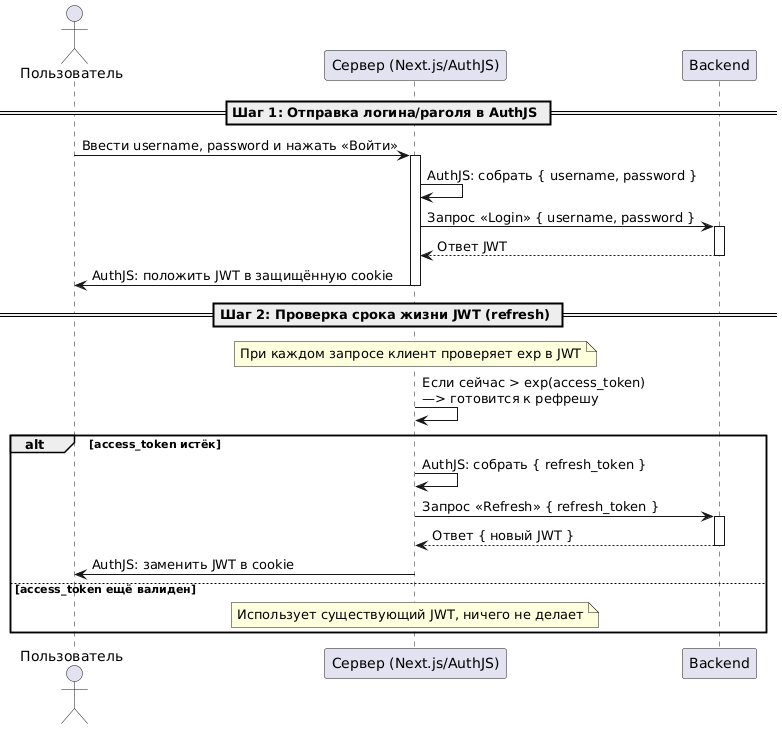
\includegraphics[width=0.9\textwidth]{static/diagrams/AuthRefresh.png}
    \caption{Схема процесса проверки и обновления JWT токена через токен обновления}
    \label{fig:auth-refresh}
\end{figure}

На рисунке~\ref{fig:auth-refresh} можно выделить два основных этапа: аутентификация пользователя и процесс использования токена.

При входе пользователя в систему происходит следующая последовательность действий:
\begin{enumerate}
    \item Пользователь вводит поля \textit{username} и \textit{password} в приложение;
    \item Модуль Auth.js формирует объект с учётными данными и отправляет запрос на сервер (метод \textit{login});
    \item Сервер возвращает токен доступа и токен обновления;
    \item Модуль Auth.js сохраняет полученный JWT токен в защищённые cookie данные.
\end{enumerate}

После успешной аутентификации при каждом запросе выполняется проверка срока жизни токена и, при необходимости, его обновление.  Ниже приведены основные этапы этой проверки и процесса обновления:
\begin{enumerate}
    \item При каждом запросе клиент проверяет поле \textit{exp} (срок жизни) в токене доступа.
    \item Если текущий момент времени превысил время жизни токена доступа, начинается подготовка к обновлению токена.
    \item В случае истечения срока действия токена доступа модуль Auth.js отправляет токен обновления на сервер. Сервер возвращает новый токен доступа и новый токен обновления. После этого модуль Auth.js заменяет старый токен в cookie браузера на новый.
    \item Если же токен доступа ещё валиден, модуль Auth.js просто использует существующий токен и не делает дополнительных запросов (промежуточные уведомления внизу диаграммы).
\end{enumerate}

Таким образом, схема на рисунке~\ref{fig:auth-refresh} демонстрирует, что клиент всегда сначала пробует воспользоваться существующим токеном доступа, проверяя его валидность. Только если проверка не проходит, выполняется последовательность обновления, благодаря чему повышается отказоустойчивость и исключается ситуация «гонки» при параллельных запросах на обновление.

Важным дополнением к этой концепции является механизм предотвращения <<гонки состояний>> при одновременном запросе нескольких API-методов, обнаруживающих, что токен доступа просрочен. В таких случаях на клиенте сохраняется единственный промис обновления, который переиспользуется всеми последующими запросами до получения ответа от сервера. Пример реализации этого механизма приведён в листинге~\ref{lst:race-condition}.

\begin{lstlisting}[caption={Механизм предотвращения гонки состояний при рефреше токена}, label={lst:race-condition}]
	export type RefreshPromiseStateType = Promise<JWT | null> | null;
	let tokenPromiseState: RefreshPromiseStateType = null;
	export const setTokenPromiseState = (
		promise: RefreshPromiseStateType
	): void => {
		tokenPromiseState = promise;
	};
	export const getTokenPromiseState = (): RefreshPromiseStateType => {
		return tokenPromiseState;
	};

	let tokenState: JWT | null = null;
	export const setTokenState = (newTokenState: JWT | null): void => {
		tokenState = newTokenState;
	};
	export const getTokenState = (): JWT | null => {
		return tokenState;
	};

	let timeoutState: NodeJS.Timeout | null = null;
\end{lstlisting}

На основе приведённой логики обеспечивается централизованная обработка авторизации и обновления токенов без дублирования текста программмы в разных частях приложения. Кроме того, использование одной общей очереди запросов к серверу для обновления JWT токена предотвращает нежелательные состояния гонки и лишние обращения к серверу.
